\section{Running Example}
%
We illustrate our concepts using a three-tank system, as shown in figure~\ref{fig:three_tanks}. The
tanks are denoted as $T_1$, $T_2$, and $T_3$. They all have the same
area $A_1 = A_2 = A_3 = 3~[\textrm{m}^2]$. The three tanks are
indestructible and of infinite height representing an idealized
experiment.  We assume that $g = 10$ and the liquid is ``pure'' water
with density $\rho = 1$.
%
\begin{figure}[htb]
  \centering
  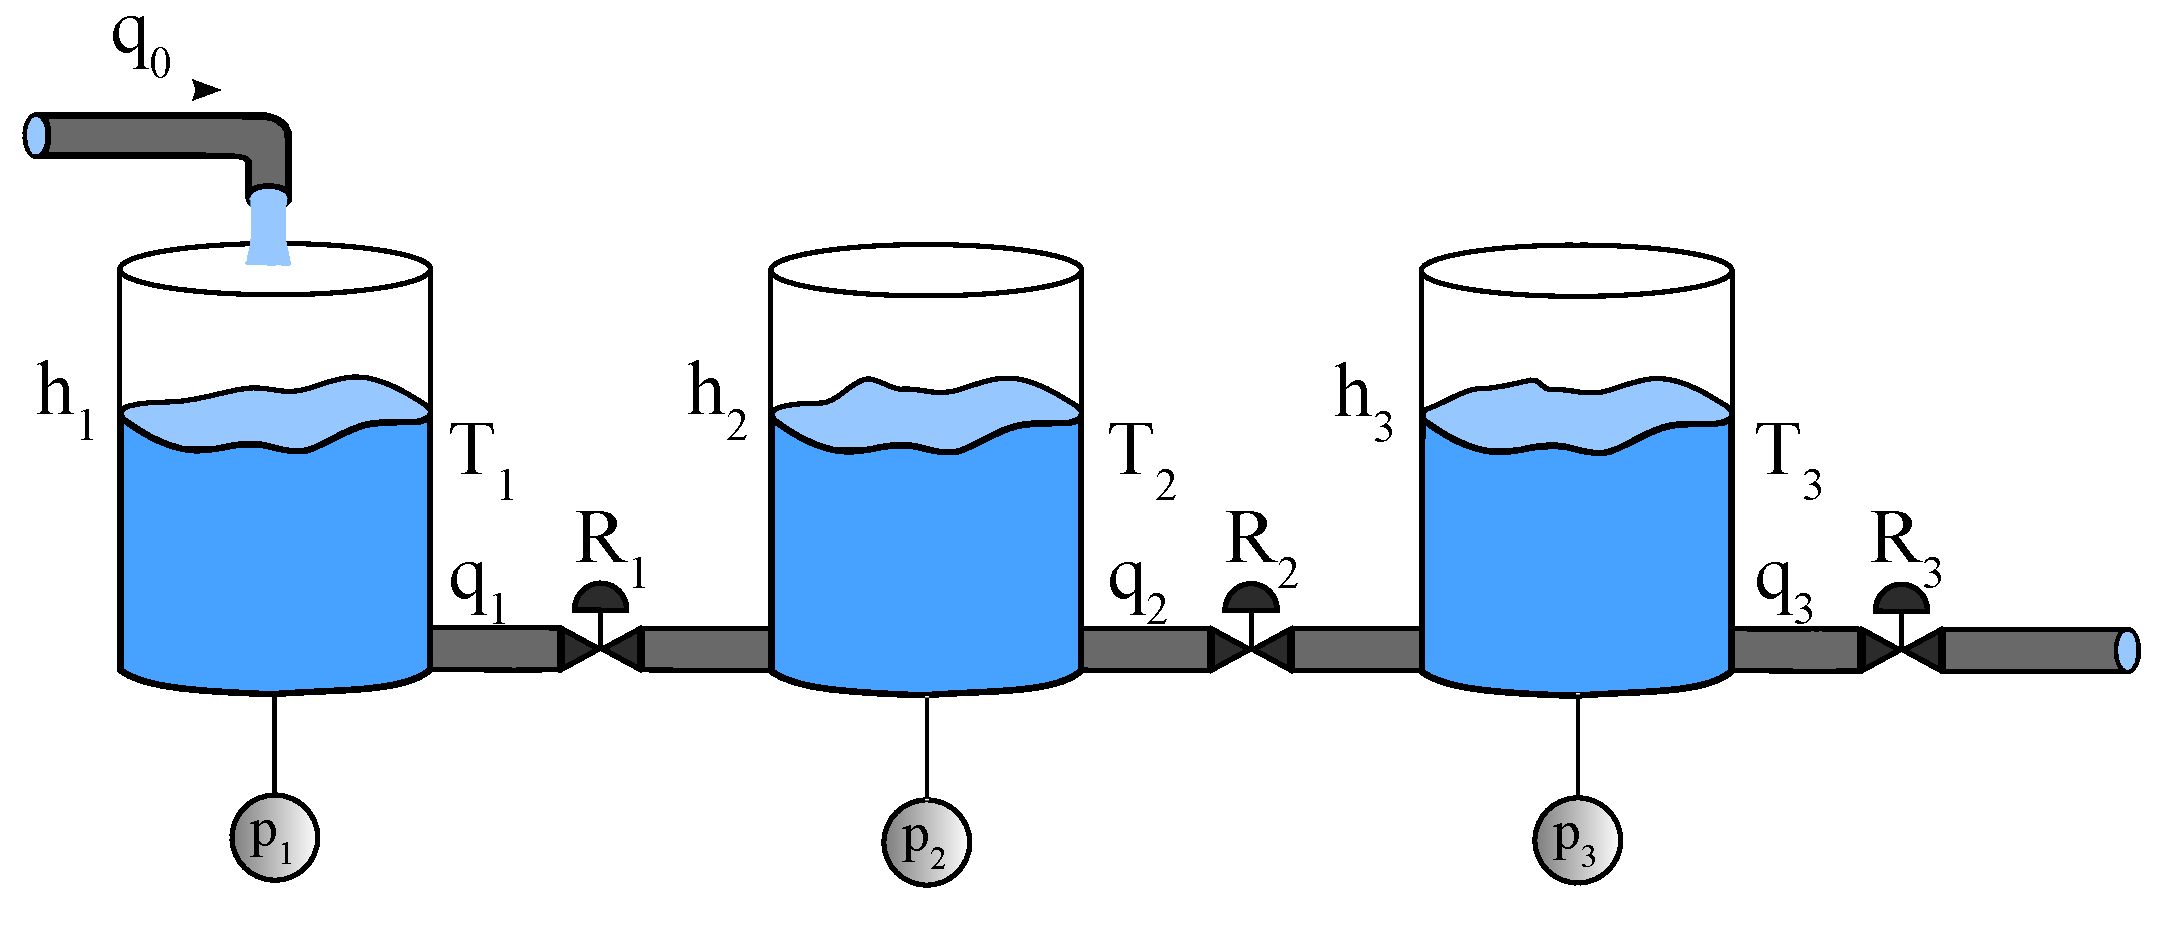
\includegraphics[width=1\columnwidth]{3-tanks}
  \caption{Diagram of the three-tank system.}
  \label{fig:three_tanks}
\end{figure}
\par\noindent
%
Tank $T_1$ is filled from a pipe $q_0$ with a constant flow of
$0.75~[\textrm{m}^3/\textrm{s}]$. It drains into $T_2$ via a pipe
$q_1$. The liquid level is denoted as $h_1$. There is a pressure
sensor $p_1$ connected to $T_1$ that measures the pressure in Pascals
[Pa]. Starting from Newton's (and Bernouli's) equations and
manipulating them (the actual derivation is irrelevant in this paper)
we derive the following Ordinary Differential Equation (ODE) that
gives the level of the liquid in $T_1$:
%
\begin{eqnarray}
%
\frac{d h_1}{dt} = \frac{q_0 - k_1 \sqrt{h_1 - h_2}}{A_1}\label{eq:ode1}
%
\end{eqnarray}
%
In eq.~\ref{eq:ode1}, the coefficient $k_1$ is the product of the
cross-sectional area of the tank $A_1$ and the area of the drainage
hole and $\sqrt{2g}$ and the friction/contraction factor of the
hole. We emphasize the use of $k_1$ because, later, we will be
``diagnosing'' our system in term of changes in $k_1$. Consider a
physical valve $R_1$ between $T_1$ and $T_2$ that constraints the flow
between the two tanks. We can say that the valve changes
proportionally to the cross-sectional drainage area of $q_1$ and hence
$k_1$. The diagnostic task is to compute the true value of $k_1$,
given $p_1$, and from $k_1$ we can compute the actual position of the
valve $R_1$.
%
The water levels of $T_2$ and $T_3$, denoted as $h_2$ and $h_3$
respectively, are given by:
%
\begin{eqnarray}\label{eq:tank1}
%
\frac{d h_i}{dt} = \frac{k_{i - 1} \sqrt{h_{i - 1} - h_i} - k_i \sqrt{h_i}}{A_i},
%
\end{eqnarray}
%
where $i$ is the tank index ($i \in \{2, 3\}$).
\par
We assume that $k_1 = k_2 = k_3 = 0.75$.
\par
Finally, we turn the water level into pressure:
\begin{eqnarray}
p_i = \frac{g\,h_i\,A}{A} = g\,h_i\label{eq:pressure}
\end{eqnarray}
where $i$ is the tank index ($i \in \{1, 2, 3\}$).
\par
We assume that the initial water level in the three tanks is zero.